\section{PI2-NL System Design}
\subsection{Design Overview}

\sys defines a concrete set of \difftree syntax as an intermediate representation between natural language tasks and data visualizations. The advantage of \difftree representations over SQL queries is that natural language utterances often contain ambiguities that are hard to be encoded into a single SQL query, and a \difftree is more capable of capturing these ambiguities and is better aligned with \sysold 's visualization interfaces.

For instance, a natural language task "How badly has covid impacted the Seattle area?" could be translated into the following \difftree : select time, ANY(covid\_cases, covid\_deaths) from covid where city = ANY('Seattle', 'Bellevue', 'Tukwila', 'Redmond', 'Tacoma', 'Bothell'); and the two ANY choice nodes could later be mapped to dropdown widgets in the visualization interface. The complete set of \difftree syntax will be discussed in the following section.

\sys leverages the few-shot performance of Codex to produce \difftrees with only a few examples provided in the prompt. We used 50 examples with 5 different database schemata to teach Codex NL-to-\difftree translation. Then, we prompt Codex with a natural language task and the task's database schema to generate a \difftree representation, which would then be used as an input for \sysold to produce interactive data visualizations.

\begin{figure*}
    \centering
    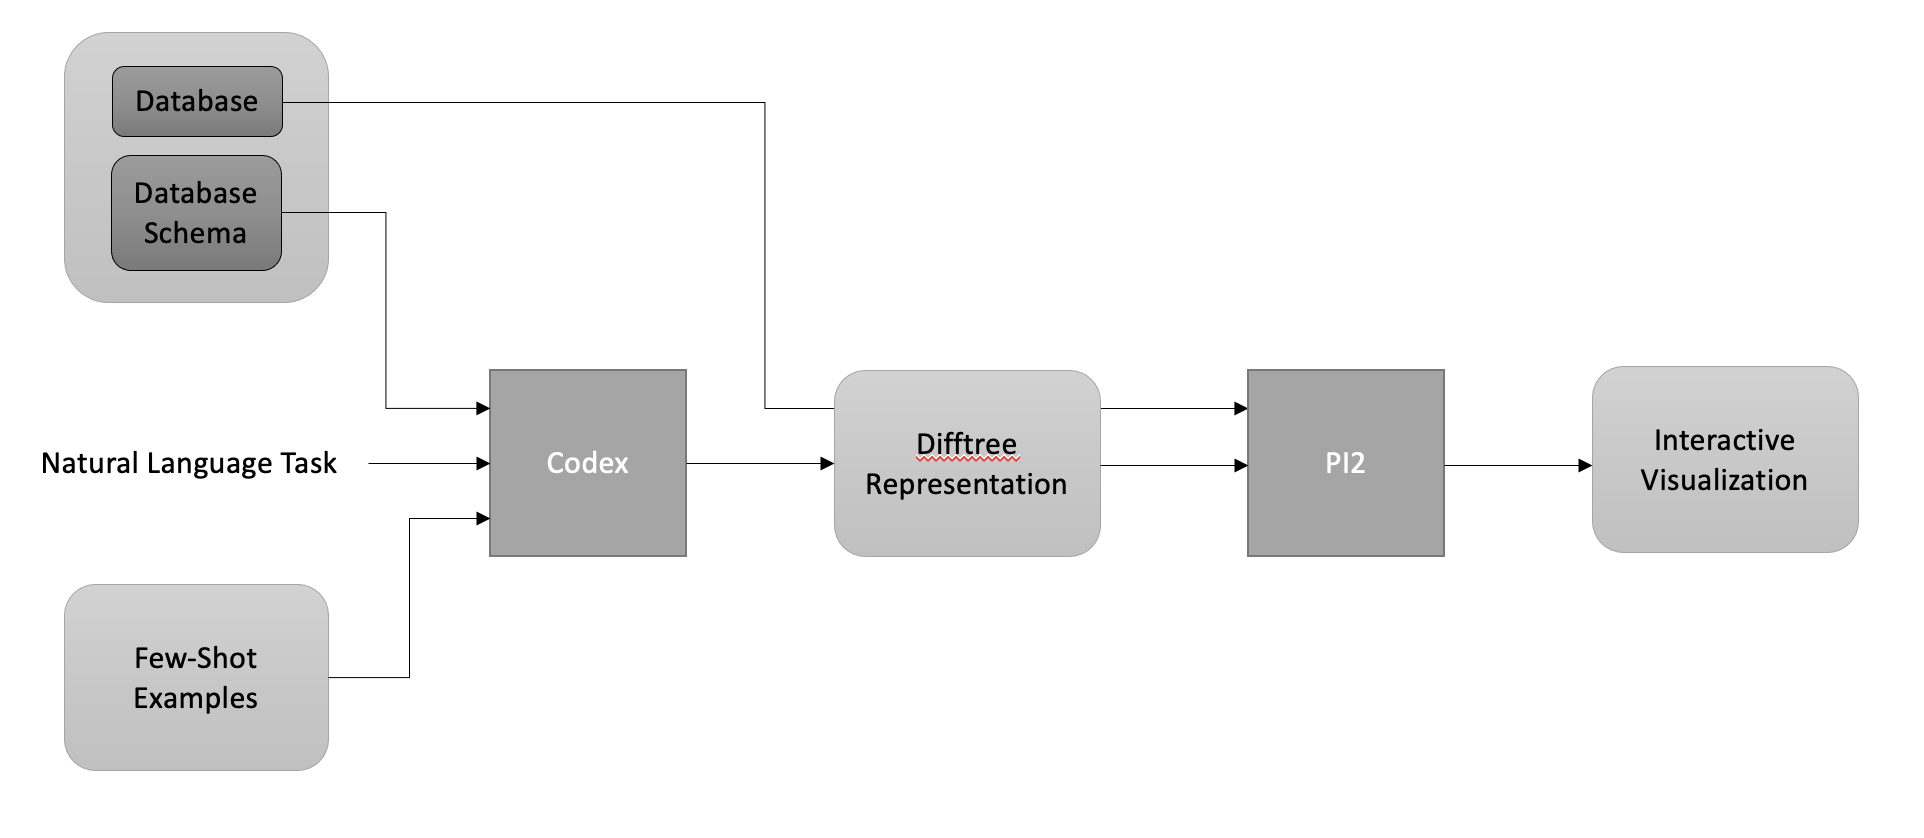
\includegraphics[width=0.8\textwidth]{nlviz-workshop/figure/pipline.png}
    \caption{The complete pipeline for generating interactive interfaces from a natural language task}
    \label{fig:pipline}
\end{figure*}


\subsection{\difftree Representation}

\difftrees were first introduced by PI2\cite{chen2022pi2} to encode the semantic variations among multiple SQL queries. However, there wasn't a well-defined textual representation of \difftree that could be used to transmit among multiple systems. Our paper proposes a formal set of syntax to write a \difftree as text or parse a \difftree from textual input.

\difftree input strings are a strict superset of the traditional SQL language. In addition to the standard SQL syntax, \difftree introduces choice nodes to provide the freedom and capacity to encode more information than a single SQL query. These choice nodes are:

\begin{enumerate}
\item $\mathbf{ANY(c1, ..., ck) \rightarrow c1 \vee ... \vee ck}$. The ANY choice node allows one to select any one of the values enclosed by the parentheses. To specify a range of numeric values, one can instead use $\mathbf{ANY(a - b)}$; e.g., $\mathbf{ANY(3.0 - 5.0)}$ represents any numeric value between 3.o and 5.0. Moreover, it is sometimes beneficial to include a default value in an ANY choice node (e.g., to instruct PI2 setting a default value for a dropdown widget). A default value can be specified by using the 'default' keyword: $\mathbf{ANY(c1, ..., ck, default=ci)}$
\item $\mathbf{SUBSET(c1, ..., ck) \rightarrow c1? \cup ... \cup ck?}$. As the name suggests, the SUBSET choice node specifies a subset of the values listed between the parentheses. For example, the query "select col1, col2 from table1 where $\mathbf{SUBSET(c1, ..., ck)}$" represents all SQL queries that selects col1 and col2 from table1 with any combinations of c1, ..., ck in the where clause.
\item $\mathbf{OPT(t) \rightarrow t \vee NULL}$. The OPT choice node implies that the term in the parentheses is optional in the query. For instance, \difftree query "select col1, col2 from table1 where c1 and $\mathbf{OPT(c2)}$" encodes both SQL query "select col1, col2 from table1 where c1" and "select col1, col2 from table1 where c1 and c2". \difftree query "select col1, OPT(col2) from table1" represents both "select col1 from table1" and "select col1, col2 from table1".
\end{enumerate}

We note that since \difftrees are a strict superset of SQL queries, regular SQL queries are also considered to be valid inputs for the \difftree parser.